\documentclass[a4paper, 12pt]{article}
\usepackage{ctex}
\usepackage{graphicx}
\usepackage{subfigure}
\usepackage{booktabs} %三线表
\usepackage[unicode]{hyperref}
\usepackage{xcolor}
\usepackage[super,square]{natbib}
\usepackage{indentfirst}
\usepackage{amsmath}
\usepackage[ruled,vlined]{algorithm2e}
\usepackage{titlesec}
\usepackage{listings}

\lstset{ %
backgroundcolor=\color{white},   % choose the background color
basicstyle=\footnotesize\ttfamily,        % size of fonts used for the code
columns=fullflexible,
breaklines=true,                 % automatic line breaking only at whitespace
captionpos=b,                    % sets the caption-position to bottom
tabsize=4,
commentstyle=\color{mygreen},    % comment style
escapeinside={\%*}{*)},          % if you want to add LaTeX within your code
keywordstyle=\color{blue},       % keyword style
stringstyle=\color{mymauve}\ttfamily,     % string literal style
frame=single,
rulesepcolor=\color{red!20!green!20!blue!20},
% identifierstyle=\color{red},
language=c++,
}

%%%% 下面的命令重定义页面边距,使其符合中文刊物习惯 %%%%
\addtolength{\topmargin}{-54pt}
\setlength{\oddsidemargin}{0.63cm}  % 3.17cm - 1 inch
\setlength{\evensidemargin}{\oddsidemargin}
\setlength{\textwidth}{14.66cm}
\setlength{\textheight}{24.00cm}    % 24.62

%%%% 下面的命令设置行间距与段落间距 %%%%
\linespread{1.4}
% \setlength{\parskip}{1ex}
\setlength{\parskip}{0.5\baselineskip}

\begin{document}
\titleformat{\section}{\large\bfseries}{第\,\thesection\,章}{1em}{}
\bibliographystyle{plain}%abbrv,plain,alpha
%%%% 定理类环境的定义 %%%%
\newtheorem{example}{例}             % 整体编号
\newtheorem{theorem}{定理}[section]  % 按 section 编号
\newtheorem{definition}{定义}
%\newtheorem{algorithm}{算法}
\newtheorem{axiom}{公理}
\newtheorem{property}{性质}
\newtheorem{proposition}{命题}
\newtheorem{lemma}{引理}
\newtheorem{corollary}{推论}
\newtheorem{remark}{注解}
\newtheorem{condition}{条件}
\newtheorem{conclusion}{结论}
\newtheorem{assumption}{假设}

%%%% 重定义 %%%%
\renewcommand{\contentsname}{目录}  % 将Contents改为目录
%\renewcommand{\abstractname}{摘要}  % 将Abstract改为摘要
\renewcommand{\refname}{参考文献}   % 将References改为参考文献
\renewcommand{\indexname}{索引}
\renewcommand{\figurename}{图}
\renewcommand{\tablename}{表}
\renewcommand{\appendixname}{附录}
\renewcommand{\algorithmcfname}{算法} %针对 algorithm2e 宏包

%%%% 定义标题格式,包括title,author,affiliation,email等 %%%%
\title{基于成本加成理论的政府对新能源汽车补贴的分析}
\author{李勇奇\\
 同济大学控制科学与工程系,上海,201804;\\[2ex]}
\date{2016年1月}

% \maketitle

% \begin{abstract}
%   阐述成本加成或成本加价的理论、方法、基本模型,结合我国目前政府对新能源汽车购车予以补贴的实际情况,试写出修正的成本加价模型并进行分析
%   \\
%   \textbf{关键字:} 成本加成~~新能源汽车~~循环矩阵~~目标追踪
% \end{abstract}

\tableofcontents
\newpage
\section{引言}
GPS(Global Positioning System)是全球定位系统,是由美国国防部研制建立的一种具有全方位、全天候、全时段、高精度的卫星导航系统,能为全球用户提供低成本、高精度的三维位置、速度和精确定时等导航信息,是卫星通信技术在导航领域的应用典范,它极大地提高了地球社会的信息化水平,有力地推动了数字经济的发展。

本文主要专注于GPS模型块的使用,包括GPS数据的读取与解析,数据的滤波,以及利用GPS数据计算运动的距离,与地图相连接等,最终将上述功能结合在一起利用Python语言编写了一个具有图形界面的应用程序。

\section{GPS 数据解析与应用}
由于手头的GPS是已经封装好的模块,所以本文主要侧重于GPS模块软件方面的应用,包括对GPS模块传回的数据的解析、Kalman滤波以及利用GPS计算移动的距离。

\subsection{GPS 数据格式}
GPS模块上电之后每隔一段事件都会从串口传回如下固定格式的数据:
\begin{lstlisting}
    $GPGGA,235949.042,0000.0000,N,00000.0000,E,0,00,,0.0,M,0.0,M,,0000*45
    $GPGLL,0000.0000,N,00000.0000,E,235949.042,V,N*47
    $GPGSA,A,1,,,,,,,,,,,,,,,*1E
    $GPGSV,1,1,00*79
    $GPRMC,235949.042,V,0000.0000,N,00000.0000,E,,,140209,,,N*7E
    $GPVTG,,T,,M,,N,,K,N*2C
\end{lstlisting}
该数据格式符合NMEA-0813x协议,NMEA 0183是美国国家海洋电子协会(National Marine Electronics Association )为海用电子设备制定的标准格式。目前业已成了GPS导航设备统一的RTCM(Radio Technical Commission for Maritime services)标准协议。其数据类型主要有以下六种:
\begin{itemize}
\item GPGSV:可见卫星信息
\item GPGLL:地理定位信息
\item GPRMC:推荐最小定位信息
\item GPVTG:地面速度信息
\item GPGGA:GPS定位信息
\item GPGSA:当前卫星信息
\end{itemize}
为了获得GPS的时间、经度、纬度和地面速率,查阅协议可以发现所要获得的数据可以从GPRMC和GPGGA提取到,以GPRMC数据为例,其数据标准格式如下:
\begin{lstlisting}
\$GPRMC,<1>,<2>,<3>,<4>,<5>,<6>,<7>,<8>,<9>,<10>,<11>,<12>*hh
\end{lstlisting}
其中:\\
<1> UTC 时间,hhmmss(时分秒)格式\\
<2> 定位状态,A=有效定位,V=无效定位\\
<3> 纬度ddmm.mmmm(度分)格式(前面的0也将被传输)\\
<4> 纬度半球N(北半球)或S(南半球)\\
<5> 经度dddmm.mmmm(度分)格式(前面的0也将被传输)\\
<6> 经度半球E(东经)或W(西经)\\
<7> 地面速率(000.0~999.9节,前面的0也将被传输)\\
<8> 地面航向(000.0~359.9度,以真北为参考基准,前面的0也将被传输)\\
<9> UTC 日期,ddmmyy(日月年)格式\\
<10> 磁偏角(000.0~180.0度,前面的0也将被传输)\\
<11> 磁偏角方向,E(东)或W(西)\\
<12> 模式指示(仅NMEA01833.00版本输出,A=自主定位,D=差分,E=估算,N=数据无效)\\
根据上述信息,要获得时间、经度、纬度和速率信息只要提取相应位的数据以及相应的单位转换。

其他数据类型此处不再详细介绍,参考相关数据手册即可。

\subsection{Kalman 滤波}
为了更准确的获得经度纬度信息,采用Kalman滤波算法对GPS返回的经度纬度和地面速率进行滤波。Kalman滤波算法是一种最优化自回归数据处理算法,其原理和具体公式推导此处不详细描述,直接给出其时间和状态的更新方程。
\begin{itemize}
\item 时间更新方程:
  \begin{eqnarray}
    \label{eq:1}
    &&\hat{\mathbf{X}}_k^- = \mathbf{A}\hat{\mathbf{X}}_{k-1} + \mathbf{B}\hat{\mathbf{U}}_{k-1}\\
    &&\mathbf{P}_k^- = \mathbf{A}\mathbf{P}_{k-1}\mathbf{A}^T + \mathbf{Q}
  \end{eqnarray}
\item 状态更新方程:
  \begin{eqnarray}
    \label{eq:2}
    &&\mathbf{K}_k = \mathbf{P}_k^-\mathbf{H}^T(\mathbf{H}\mathbf{P}_k^- + \mathbf{R})^{-1}\\
    &&\hat{\mathbf{X}}_k = \hat{\mathbf{X}}_k^- + \mathbf{K}_k(\mathbf{Z}_k-\mathbf{H}\hat{\mathbf{X}}_k)\\
    &&\mathbf{P}_k = (\mathbf{I} - \mathbf{K}_k\mathbf{H})\mathbf{P}_k^-
  \end{eqnarray}
\end{itemize}
上述时间和状态更新方程是对于多维变量的矩阵形式,由于本文所需要的数据较为简单,控制变量$\mathbf{U}=0$,且认为经度纬度和速度并不相关,则将上述Kalman更新方程简化为一维形式。
\begin{itemize}
\item 时间更新方程:
  \begin{eqnarray}
    \label{eq:3}
    &&\hat{x}_k^- = \hat{x}_{k-1}\\
    &&p_k^- = p_{k-1} + Q\\
  \end{eqnarray}
\item 状态更新方程:
  \begin{eqnarray}
    \label{eq:4}
    && k_k = p_k^-/(p_k^- + R)\\
    &&\hat{x}_k = \hat{x}_k^-+k_k(z_k-\hat{x}_k)\\
    &&p_k = (1-k_k)p_k^-
  \end{eqnarray}
\end{itemize}
其中$z$表示观测变量,$\hat{x}$表示状态变量的后验估计,$\hat{x}^-$表示状态变量的先验估计,$\hat{p}$表示误差的后验估计,$\hat{p}^-$表示误差的先验估计,$Q$表示误差方差,$R$表示测量方差。简单来说,以经度为例,GPS返回的经度值就是$z_k$,经过Kalman滤波,返回滤波后的经度值是$\hat{x}_k$。

\subsection{距离解算}
根据GPS返回的数据可以计算运动路径中两点的距离,利用返回的时间、经度、纬度和地面速率信息可以想到两种计算距离的方法。较为简单的是利用速率对时间积分,因为GPS每个一小段时间$\Delta t_k$都会返回一个速率$v_k$,则距离的可由以下公式计算得到
\begin{equation}
  \label{eq:5}
  D_{ij} = \sum_{k=i}^j{\Delta t_k \times v_k}
\end{equation}

另一种计算距离的方法可以通过经度纬度信息得到,计算公式如下:
\begin{equation}
  \label{eq:6}
  D_{ij} = \sum_{k=i}^j{\sqrt{(rcos(\frac{\alpha_{k-1}+\alpha_k}{2})(\beta_k-\beta_{k-1}))^2+(r(\beta_k-\beta_{k-1}))^2}}
\end{equation}
其中$\alpha$、$\beta$分别表示纬度和经度,$r$表示地球半径。其原理就是利用微积分的思想计算球面上两点的距离。

\section{软件模块设计}
软件模块主要完成的功能是实时显示经纬度、运动距离等信息,并在在地图上实时显示位置,主要包括四个模块:
\begin{itemize}
\item GPS模块
\item Kalman滤波模块
\item map模块
\item GUI模块
\end{itemize}
软件模块整体的构架如图\ref{fig:2}所示。
\begin{figure}[ht]
  \centering
  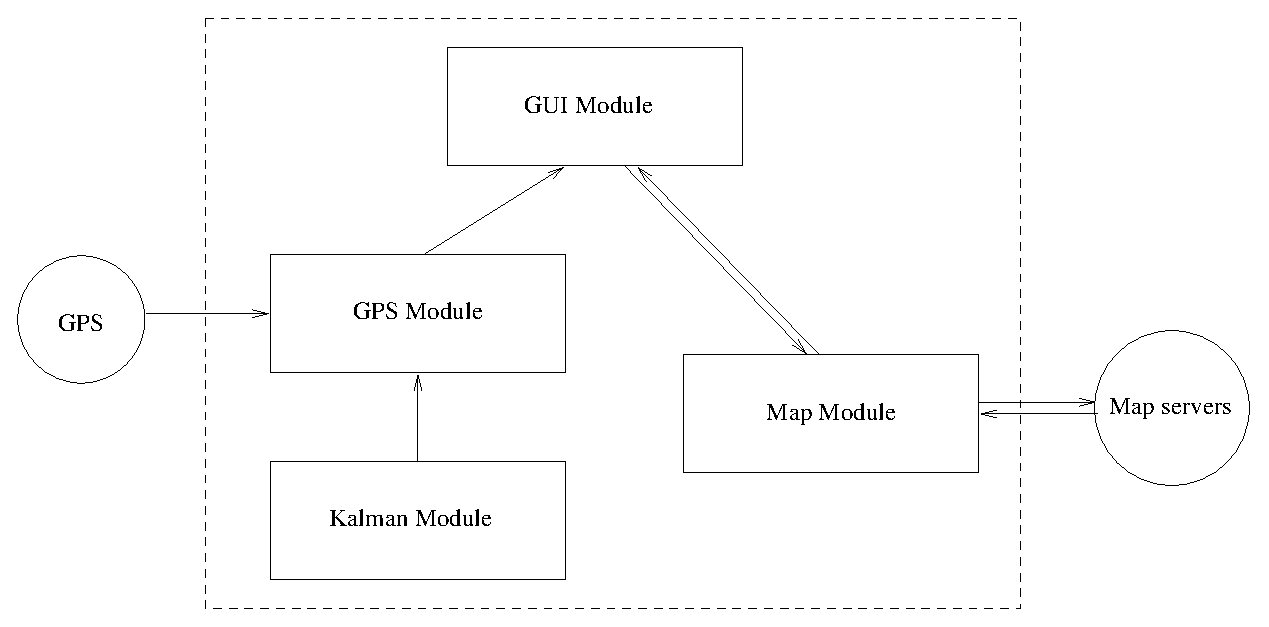
\includegraphics[width=15cm]{f2.eps}
  \caption{软件模块整体构架}
  \label{fig:2}
\end{figure}
其中虚线框内为所设计的软件模块,圆形GPS表示实际的GPS,Map servers表示提供地图服务的服务器,如Google的地图服务和百度的地图服务。矩形框内表示四个软件模块,Kalman模块提供一个Kalman滤波器方便GPS模块调用;GPS模块主要从实际的GPS中读取数据,然后对数据进行解析,并提供计算运动距离的方法,最后调用Kalman滤波器对数据进行滤波;Map模块主要负责通过互联网和提供地图服务的服务器进行交互,比如可以调用百度地图api向其服务器请求指定经纬度的静态图,然后向GUI模块提供指定经纬度的静态图;GUI模块负责整个程序图形界面的显示,以及将各个模块整合在一起。具体各个模块的实现细节见下文。

\subsection{开发环境}
软件的开发是在Linux下使用Python语言编写的,具体信息如表\ref{tab:1}所示。
\begin{table}[ht]
  \centering
  \caption{软件开发环境}
  \label{tab:1}
  \begin{tabular}{lc}
    \toprule
    操作系统 & Ubuntu 14.04.3 LTS x86\_64\\
    程序语言 & Python 2.7.6\\
    编辑器 & Emacs 24.5\\
    版本控制 & git 2.6.4\\
    \bottomrule
  \end{tabular}
\end{table}
选择Python作为开发语言一方面是因为时间比较紧,而Python作为一门相当高级的语言相比C有较高的开发效率;另一方面,Python是一门面向对象语言,而且第三方库相当丰富,写GUI程序较为方便。Python的高效的开发效率的后果就是程序运行速率慢,但是对于本次实验并没有影响。

\subsection{具体实现}
对于GPS数据解析模块,其逻辑较为简单,其基本内容包括从GPS中读取原始数据,然后从原始数据中解析所需要的数据,然后解算运动的距离,再用Kalman滤波对数据滤波一下,然后提供给GUI模块。由于只要获取时间、经度、纬度和地面速率四个量,所以只要处理GPS返回数据中的\$GPRMC信息即可,然后提取相应的时间、经度、纬度和地面速率,然后计算运动距离,最后再用Kalman对数据滤波。其程序流程图如图\ref{fig:1}所示。
\begin{figure}[ht]
  \centering
  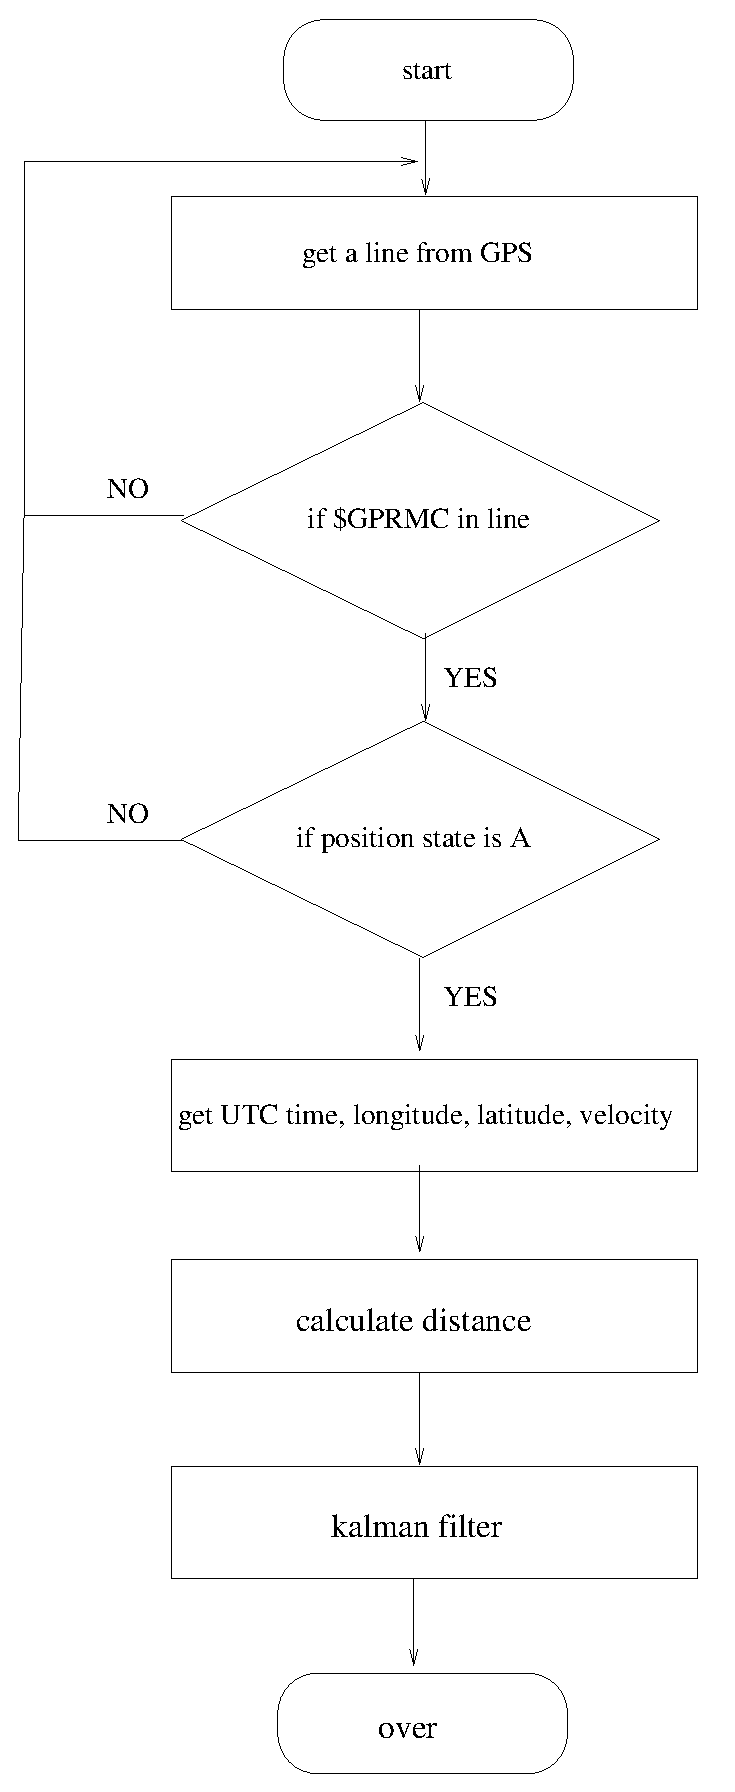
\includegraphics[width=6cm]{f1.eps}
  \caption{GPS数据解析流程图}
  \label{fig:1}
\end{figure}
调用该GPS数据解析函数一次就返回一次有效定位的时间、经度、纬度、地面速率值和运动距离。


对于Kalman滤波模块,为了增加该模块的复用和可扩展性,将其写成了一个类,其核心部分就是第二章中五个更新公式,其更新的算法如算法\ref{alg:1}所示。
\begin{algorithm}[ht]
\caption{一维Kalman 滤波数据更新算法}
\label{alg:1}
\KwIn{观察值 $z_k$}
\KwOut{滤波后的观察值$\hat{z}_k$}
初始化参数$Q$、$R$\;
\For {k=1; k<N;}
{
  // 时间更新\;
  $\hat{x}_k^- = \hat{x}_{k-1}$\;
  $p_k^- = p_{k-1} + Q$\;
  // 状态更新\;
  $k_k = p_k^-/(p_k^- + R)$\;
  $\hat{x}_k = \hat{x}_k^-+k_k(z_k-\hat{x}_k)$\;
  $p_k = (1-k_k)p_k^-$\;
  // 输出\;
  $\hat{z}_k = \hat{x}_k$\;
}
\end{algorithm}

对于map模块,其内部逻辑是首先从GUI模块出获得经度纬度信息,然后根据经度纬度信息,以及在地图服务端设置的ak和sk信息计算sn值,然后向地图服务端发送指定经度纬度的静态图,等待地图服务器传回来的图片,最后将图片返回给GUI模块。

对于GUI模块,其实现的主要功能是根据当前经度纬度等信息在图形界面实时显示以及向map模块发送请求获得当前经度纬度的静态图。该模块较为复杂,包含GUI相关部分,并且涉及到相关模块之间的通信。GUI部分采用PyQt框架,PyQt是一个创建GUI应用程序的工具包,它是Python编程语言和Qt库的成功融合,Qt是比较有名的跨平台GUI库,因此采用PyQt框架一方面可以高效的开发出GUI程序,另一方面所编写的程序也是跨平台的,只要计算机安装好Python和Qt,所编写的程序就可以在其上运行。

\section{实验结果}
所编写软件的运行画面如图\ref{fig:soft}所示。
\begin{figure}[ht]
  \centering
  \includegraphics[width=15cm]{soft.png}
  \caption{软件运行界面}
  \label{fig:soft}
\end{figure}
图中第一个下拉组合框可选择GPS的端口号,第二个下拉组合框选择波特率,按钮“open gps”根据选择的端口号和波特率打开对应端口的GPS设备,成功打开GPS后按钮标签将显示为“close gps”,另外一个“calcaulate distance”用来开始/停止计算距离。文本框显示相关信息表示当前GPS是否定位。五个标签动态显示当前的UTC时间、速度、经度、纬度和距离信息。地图是根据当前经度纬度信息向地图服务器请求的指定经度纬度的静态图,程序中每1秒向服务器请求一次,也就是说该地图每一秒刷新一次。

为了展现一下Kalman滤波的效果,滤波前和滤波后纬度值如图\ref{fig:kal}所示,该纬度信息是从华楼走到十七号楼GPS记录的纬度信息。
\begin{figure}[ht]
  \centering
  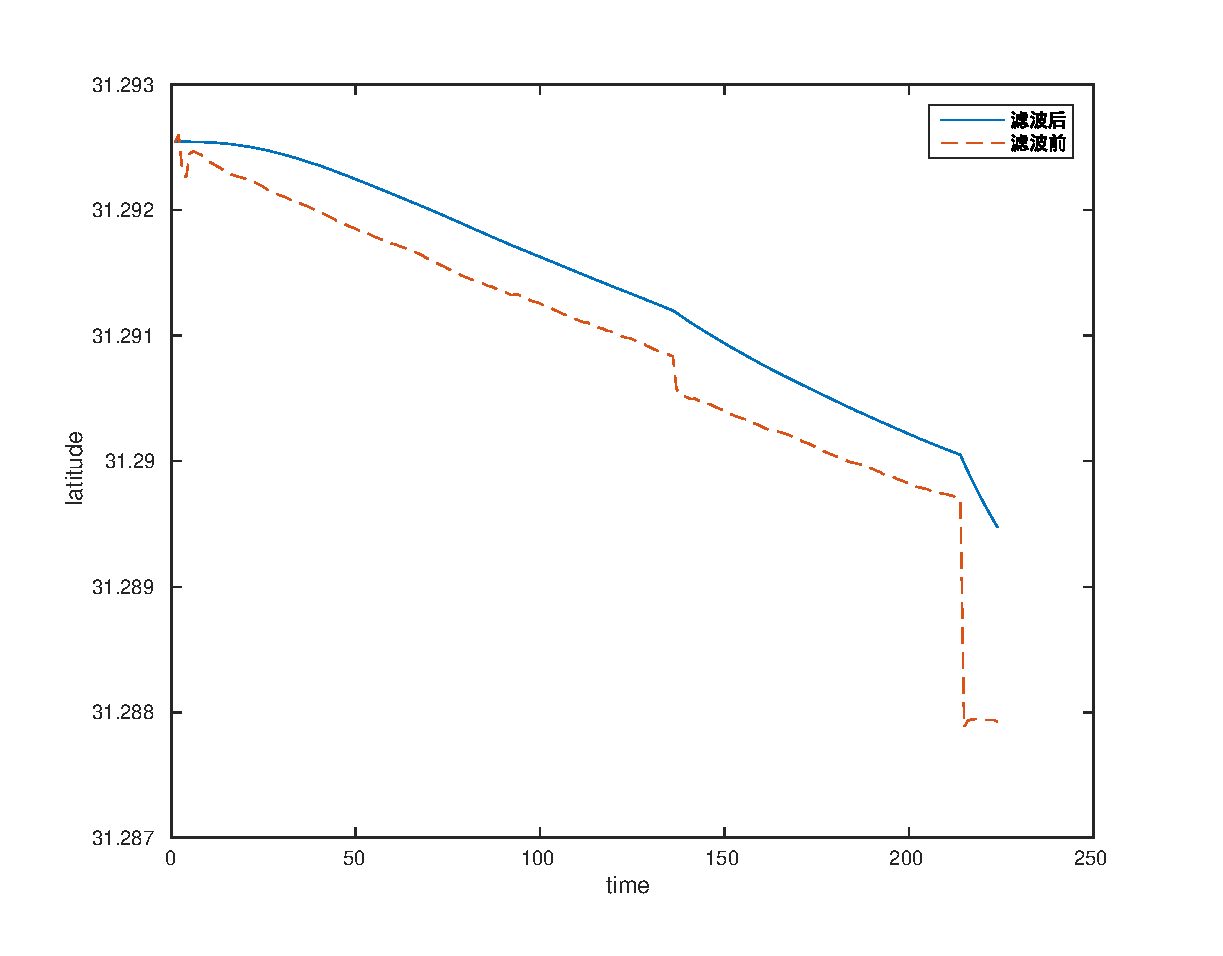
\includegraphics[width=15cm]{kal.eps}
  \caption{Kalman滤波前后纬度值}
  \label{fig:kal}
\end{figure}
从图\ref{fig:kal}可以看出Kalman滤波后的纬度比滤波前相对平滑些,由此可见Kalman滤波有一定的作用。

\section{结论}
本文在Linux平台上利用Python语言编写了一个基于GPS的应用程序,程序完成了对GPS数据的读取、解析、滤波和应用,能够实时显示当前位置、速度以及运动距离等信息,并在地图上显示当前位置。通过实际运行程序,展现了其可顺利运行,并实现相关功能。此外,对比Kalman滤波前后的数据,展现了Kalman滤波良好的效果。

\section*{致谢}
在此论文完成之际,衷心感谢苏永清老师的认真教导与帮助。

\bibliography{bib}
\end{document}